\documentclass[12pt,letterpaper]{article}
\usepackage{graphicx,textcomp}
\usepackage{natbib}
\usepackage{setspace}
\usepackage{fullpage}
\usepackage{color}
\usepackage[reqno]{amsmath}
\usepackage{amsthm}
\usepackage{fancyvrb}
\usepackage{amssymb,enumerate}
\usepackage[all]{xy}
\usepackage{endnotes}
\usepackage{lscape}
\newtheorem{com}{Comment}
\usepackage{float}
\usepackage{hyperref}
\newtheorem{lem} {Lemma}
\newtheorem{prop}{Proposition}
\newtheorem{thm}{Theorem}
\newtheorem{defn}{Definition}
\newtheorem{cor}{Corollary}
\newtheorem{obs}{Observation}
\usepackage[compact]{titlesec}
\usepackage{dcolumn}
\usepackage{tikz}
\usetikzlibrary{arrows}
\usepackage{multirow}
\usepackage{xcolor}
\newcolumntype{.}{D{.}{.}{-1}}
\newcolumntype{d}[1]{D{.}{.}{#1}}
\definecolor{light-gray}{gray}{0.65}
\usepackage{url}
\usepackage{listings}
\usepackage{color}

\definecolor{codegreen}{rgb}{0,0.6,0}
\definecolor{codegray}{rgb}{0.5,0.5,0.5}
\definecolor{codepurple}{rgb}{0.58,0,0.82}
\definecolor{backcolour}{rgb}{0.95,0.95,0.92}

\lstdefinestyle{mystyle}{
	backgroundcolor=\color{backcolour},   
	commentstyle=\color{codegreen},
	keywordstyle=\color{magenta},
	numberstyle=\tiny\color{codegray},
	stringstyle=\color{codepurple},
	basicstyle=\footnotesize,
	breakatwhitespace=false,         
	breaklines=true,                 
	captionpos=b,                    
	keepspaces=true,                 
	numbers=left,                    
	numbersep=5pt,                  
	showspaces=false,                
	showstringspaces=false,
	showtabs=false,                  
	tabsize=2
}
\lstset{style=mystyle}
\newcommand{\Sref}[1]{Section~\ref{#1}}
\newtheorem{hyp}{Hypothesis}

\title{Problem Set 3}
\date{Due: November 12, 2026}
\author{Applied Stats/Quant Methods 1}


\begin{document}
	\maketitle
	\section*{Instructions}
	\begin{itemize}
		\item Please show your work! You may lose points by simply writing in the answer. If the problem requires you to execute commands in \texttt{R}, please include the code you used to get your answers. Please also include the \texttt{.R} file that contains your code. If you are not sure if work needs to be shown for a particular problem, please ask.
	\item Your homework should be submitted electronically on GitHub.
	\item This problem set is due before 23:59 on Thursday November 12, 2026. No late assignments will be accepted.

	\end{itemize}
		\vspace{.25cm}
	
\noindent In this problem set, you will run several regressions and create an add variable plot (see the lecture slides) in \texttt{R} using the \texttt{incumbents\_subset.csv} dataset. Include all of your code.\vspace{.25cm}

\textbf{Exploring the data first:}
	\lstinputlisting[language=R, firstline=34, lastline=34]{PS03_PT.R}
		\lstinputlisting[language=R, firstline=39, lastline=42]{PS03_PT.R} 

\section*{Question 1}
\vspace{.25cm}
\noindent We are interested in knowing how the difference in campaign spending between incumbent and challenger affects the incumbent's vote share. 
	\begin{enumerate}
		\item Run a regression where the outcome variable is \texttt{voteshare} and the explanatory variable is \texttt{difflog}.
		
\lstinputlisting[language=R, firstline=46, lastline=47]{PS03_PT.R}		
\begin{verbatim}
Call:
lm(formula = inc.sub$voteshare ~ inc.sub$difflog)

Residuals:
Min       1Q   Median       3Q      Max 
-0.26832 -0.05345 -0.00377  0.04780  0.32749 

Coefficients:
Estimate Std. Error t value            Pr(>|t|)    
(Intercept)     0.579031   0.002251  257.19 <0.0000000000000002 ***
inc.sub$difflog 0.041666   0.000968   43.04 <0.0000000000000002 ***
---
Signif. codes:  0 ‘***’ 0.001 ‘**’ 0.01 ‘*’ 0.05 ‘.’ 0.1 ‘ ’ 1

Residual standard error: 0.07867 on 3191 degrees of freedom
Multiple R-squared:  0.3673,	Adjusted R-squared:  0.3671 
F-statistic:  1853 on 1 and 3191 DF,  p-value: < 0.00000000000000022	
\end{verbatim}
\textbf{Model1 shows us that on average for every one unit increase in difflog, we see about a 0.042 unit increase in vote share. A very small p value less than 0.05 allows us to reject the null hypothesis that slope = 0.}
		
		\item Make a scatterplot of the two variables and add the regression line.
\lstinputlisting[language=R, firstline=51, lastline=53]{PS03_PT.R}		
\begin{verbatim}
[1] 0.6060866
\end{verbatim}
\begin{center}
	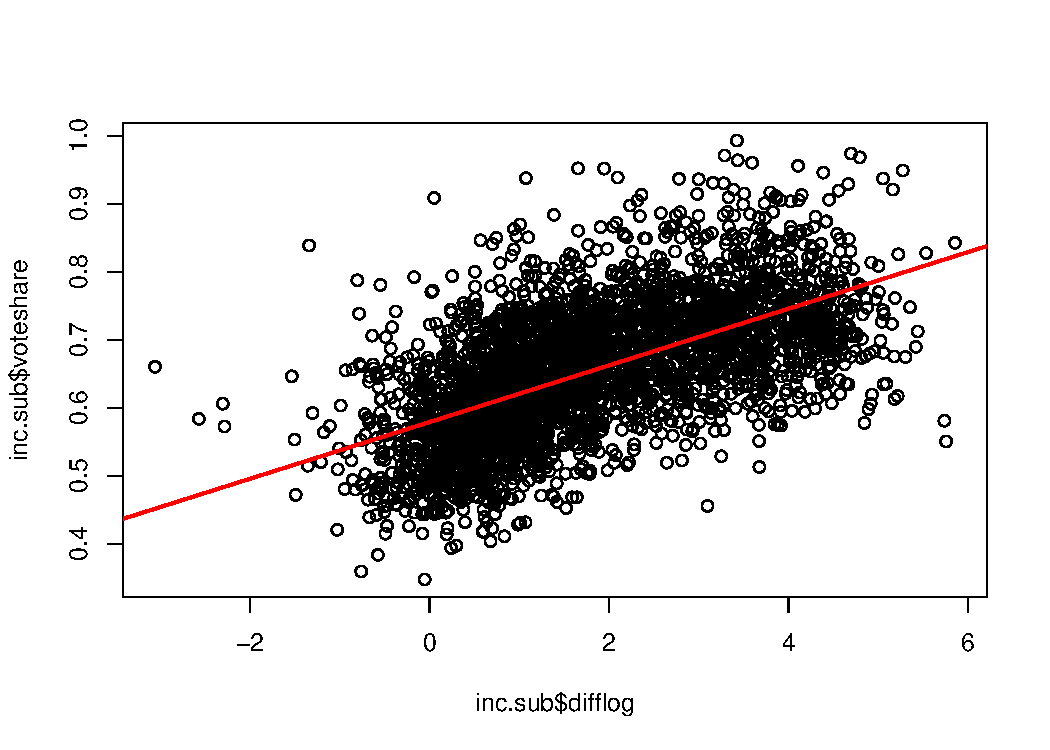
\includegraphics[width=\linewidth]{model1_plot.pdf}
\end{center}	
\textbf{The scatterplot shows a moderate positive correlation between difflog and voteshare, which is supported by the correlation coefficient r = 0.61. This indicates that incumbents who outspend their challengers have a tendency to get a higher percentage of the vote.}

		\item Save the residuals of the model in a separate object.	
\lstinputlisting[language=R, firstline=57, lastline=58]{PS03_PT.R}
\begin{verbatim}
            1             2             3             4             5             6 
-0.0004227622 -0.0316840149 -0.0045514943  0.0386688767  0.0355287965  0.0322832521 
\end{verbatim}
\textbf{The residuals are the difference between the incumbents actual vote share and their predicted vote share. These show part of voteshare that difflog did not explain. }
		\item Write the prediction equation.
\textbf{predicted voteshare = 0.579 + 0.042 * difflog}
\lstinputlisting[language=R, firstline=63, lastline=65]{PS03_PT.R}
\begin{verbatim}
[1] 0.6027841 0.6153208 0.5968093 0.6605535 0.6064495 0.5934877
\end{verbatim}
\textbf{On average, an incumbent who spends the same amount of the challenger (y-intercept, difflog = 0) is expected to get about a 0.579 share of the vote, and each one unit increase in difflog is predicted to raise about 0.042 units of voteshare.}
	\end{enumerate}
	
\newpage

\section*{Question 2}
\noindent We are interested in knowing how the difference between incumbent and challenger's spending and the vote share of the presidential candidate of the incumbent's party are related.	\vspace{.25cm}
	\begin{enumerate}
\item Run a regression where the outcome variable is \texttt{presvote} and the explanatory variable is \texttt{difflog}.
		
		\lstinputlisting[language=R, firstline=75, lastline=76]{PS03_PT.R}		
		\begin{verbatim}
Call:
lm(formula = inc.sub$presvote ~ inc.sub$difflog)

Residuals:
Min       1Q   Median       3Q      Max 
-0.32196 -0.07407 -0.00102  0.07151  0.42743 

Coefficients:
Estimate Std. Error t value            Pr(>|t|)    
(Intercept)     0.507583   0.003161  160.60 <0.0000000000000002 ***
inc.sub$difflog 0.023837   0.001359   17.54 <0.0000000000000002 ***
---
Signif. codes:  0 ‘***’ 0.001 ‘**’ 0.01 ‘*’ 0.05 ‘.’ 0.1 ‘ ’ 1

Residual standard error: 0.1104 on 3191 degrees of freedom
Multiple R-squared:  0.08795,	Adjusted R-squared:  0.08767 
F-statistic: 307.7 on 1 and 3191 DF,  p-value: < 0.00000000000000022
		\end{verbatim}
		\textbf{Model2 shows us that on average for every one unit increase in difflog, we see about a 0.024 unit increase in presvote. A very small p value less than 0.05 allows us to reject the null hypothesis that slope = 0.}
		
\item Make a scatterplot of the two variables and add the regression line.
		
		\lstinputlisting[language=R, firstline=80, lastline=82]{PS03_PT.R}		
		\begin{verbatim}
[1] 0.2965653
		\end{verbatim}
		\begin{center}
			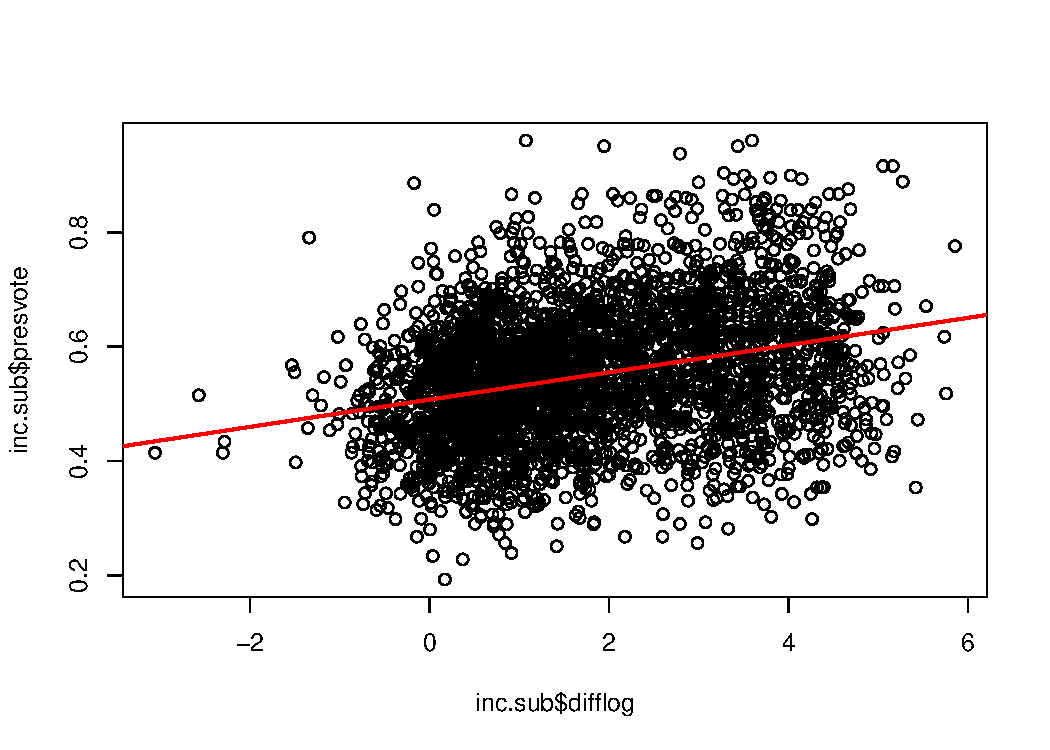
\includegraphics[width=\linewidth]{model2_plot.pdf}
		\end{center}
		\textbf{The scatterplot shows a weak to moderate positive correlation between difflog and presvote, which is supported by the correlation coefficient r = 0.3. This indicates that the presidential party candidates of incumbents who outspend their challengers have a tendency to get a higher percentage of the vote share.}
		
\item Save the residuals of the model in a separate object.
	
		\lstinputlisting[language=R, firstline=86, lastline=87]{PS03_PT.R}
		\begin{verbatim}
           1            2            3            4            5            6 
0.005605594  0.037578519 -0.053134788 -0.052993694 -0.045842994  0.074339701 
		\end{verbatim}	
		\textbf{The residuals are the difference between the presidential candidates actual vote share and their predicted vote share. These show part of presvote that difflog did not explain. }
		
\item Write the prediction equation.
		
		\textbf{predicted presvote = 0.51 + 0.024 * difflog}
		\lstinputlisting[language=R, firstline=92, lastline=94]{PS03_PT.R}
		\begin{verbatim}
[1] 0.5211726 0.5283448 0.5177544 0.5542224 0.5232696 0.5158542
		\end{verbatim}
		\textbf{On average, the party presidential candidate of an incumbent who spends the same amount of the challenger (y-intercept, difflog = 0) is expected to get about a 0.51 share of the vote, and each one unit increase in difflog is predicted to raise about 0.024 units of presvote.}
		
	\end{enumerate}

	\newpage	
\section*{Question 3}

\noindent We are interested in knowing how the vote share of the presidential candidate of the incumbent's party is associated with the incumbent's electoral success.

	\begin{enumerate}
		\item Run a regression where the outcome variable is \texttt{voteshare} and the explanatory variable is \texttt{presvote}.

\lstinputlisting[language=R, firstline=104, lastline=105]{PS03_PT.R}		
\begin{verbatim}
Call:
lm(formula = inc.sub$voteshare ~ inc.sub$presvote)

Residuals:
Min       1Q   Median       3Q      Max 
-0.27330 -0.05888  0.00394  0.06148  0.41365 

Coefficients:
Estimate Std. Error t value            Pr(>|t|)    
(Intercept)      0.441330   0.007599   58.08 <0.0000000000000002 ***
inc.sub$presvote 0.388018   0.013493   28.76 <0.0000000000000002 ***
---
Signif. codes:  0 ‘***’ 0.001 ‘**’ 0.01 ‘*’ 0.05 ‘.’ 0.1 ‘ ’ 1

Residual standard error: 0.08815 on 3191 degrees of freedom
Multiple R-squared:  0.2058,	Adjusted R-squared:  0.2056 
F-statistic:   827 on 1 and 3191 DF,  p-value: < 0.00000000000000022
\end{verbatim}
\textbf{Model3 shows us that on average for every one unit increase in presvote, we see about a 0.388 unit increase in voteshare. A very small p value less than 0.05 allows us to reject the null hypothesis that slope = 0.}

		\item Make a scatterplot of the two variables and add the regression line. 

\lstinputlisting[language=R, firstline=110, lastline=112]{PS03_PT.R}		
\begin{verbatim}
[1] 0.4536672
\end{verbatim}
\begin{center}
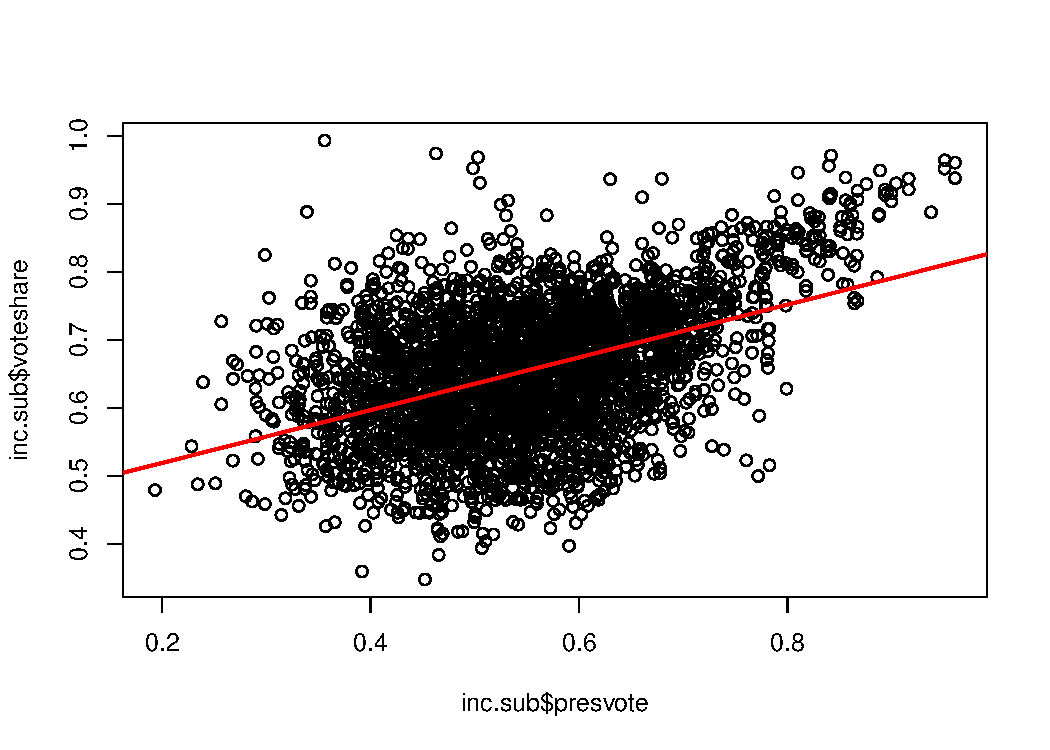
\includegraphics[width=\linewidth]{model3_plot.pdf}
\end{center}
\textbf{The scatterplot shows a moderate positive correlation between voteshare and presvote, which is supported by the correlation coefficient r = 0.454. This indicates that the incumbents have a tendency to do better when their parties presidential candidate also does better.}

		\item Write the prediction equation.

\textbf{predicted voteshare = 0.441 + 0.388 * presvote}
\lstinputlisting[language=R, firstline=117, lastline=119]{PS03_PT.R}
\begin{verbatim}
[1] 0.6457295 0.6609186 0.6216109 0.6358159 0.6265802 0.6703360
\end{verbatim}
\textbf{On average, the predicted voteshare of an incumbent whos party presidential candidate who hypothetically received none of the vote (y-intercept, presvote = 0) is expected to get about a 0.441 share of the vote, and each one unit increase in presvote is predicted to raise about 0.388 units of voteshare.}
		
	\end{enumerate}
	

\newpage	
\section*{Question 4}
\noindent The residuals from part (a) tell us how much of the variation in \texttt{voteshare} is $not$ explained by the difference in spending between incumbent and challenger. The residuals in part (b) tell us how much of the variation in \texttt{presvote} is $not$ explained by the difference in spending between incumbent and challenger in the district.
	\begin{enumerate}
		\item Run a regression where the outcome variable is the residuals from Question 1 and the explanatory variable is the residuals from Question 2.	
		
\lstinputlisting[language=R, firstline=131, lastline=134]{PS03_PT.R}		
\begin{verbatim}

Call:
lm(formula = model1_resid ~ model2_resid)

Residuals:
Min       1Q   Median       3Q      Max 
-0.25928 -0.04737 -0.00121  0.04618  0.33126 

Coefficients:
Estimate Std. Error t value Pr(>|t|)    
(Intercept)  -5.934e-18  1.299e-03    0.00        1    
model2_resid  2.569e-01  1.176e-02   21.84   <2e-16 ***
---
Signif. codes:  0 ‘***’ 0.001 ‘**’ 0.01 ‘*’ 0.05 ‘.’ 0.1 ‘ ’ 1

Residual standard error: 0.07338 on 3191 degrees of freedom
Multiple R-squared:   0.13,	Adjusted R-squared:  0.1298 
F-statistic:   477 on 1 and 3191 DF,  p-value: < 2.2e-16
\end{verbatim}
\textbf{Model4 shows us that on average for every one unit increase in model2 residuals, we see about a 0.257 unit increase in model1 residuals. A very small p value less than 0.05 allows us to reject the null hypothesis that slope = 0.}
		
		\item Make a scatterplot of the two residuals and add the regression line. 
		
\lstinputlisting[language=R, firstline=138, lastline=140]{PS03_PT.R}		
\begin{verbatim}
[1] 0.3606073
\end{verbatim}
\begin{center}
	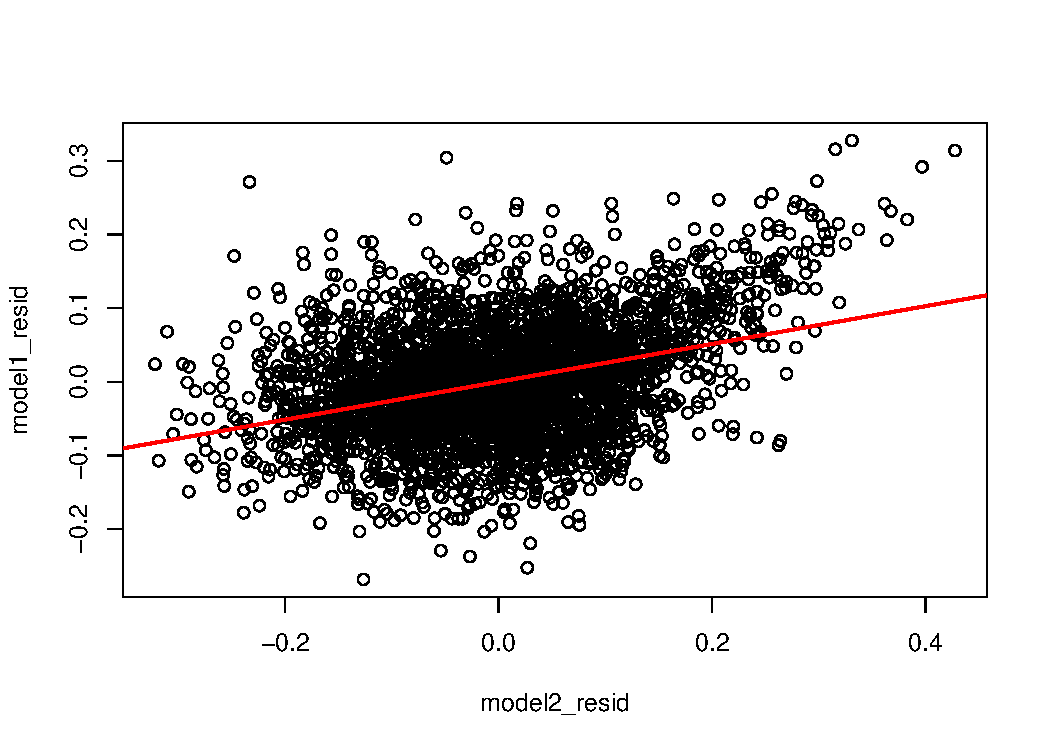
\includegraphics[width=\linewidth]{model4_plot.pdf}
\end{center}
\textbf{The scatterplot shows a weak to moderate positive correlation between model1 residuals and model2 residuals, which is supported by the correlation coefficient r = 0.36. This indicates that an increase in residuals for model1 is associated with an increase in residuals for model2. This scatterplot shows the relationship between presvote and voteshare after having removed the effect from difflog.}
		
		\item Write the prediction equation.
		
\textbf{model1 residuals = -0.000000000000000005934 + 0.257 * model2 residuals}
\lstinputlisting[language=R, firstline=145, lastline=147]{PS03_PT.R}
\begin{verbatim}
           1            2            3            4            5            6 
0.001439948  0.009653058 -0.013649106 -0.013612862 -0.011776011  0.019096160 
\end{verbatim}
\textbf{On average, the model1 residual when model2 has no residual (y-intercept, model2 residual = 0) is expected to be basically 0, and each one unit increase in model2 residuals is predicted to raise about 0.257 units of model1 residuals.}

	\end{enumerate}
	
	\newpage	

\section*{Question 5}
\noindent What if the incumbent's vote share is affected by both the president's popularity and the difference in spending between incumbent and challenger? 
	\begin{enumerate}
		\item Run a regression where the outcome variable is the incumbent's \texttt{voteshare} and the explanatory variables are \texttt{difflog} and \texttt{presvote}.	
		
\lstinputlisting[language=R, firstline=157, lastline=158]{PS03_PT.R}
\begin{verbatim}
Call:
lm(formula = inc.sub$voteshare ~ inc.sub$difflog + inc.sub$presvote)

Residuals:
Min       1Q   Median       3Q      Max 
-0.25928 -0.04737 -0.00121  0.04618  0.33126 

Coefficients:
Estimate Std. Error t value            Pr(>|t|)    
(Intercept)      0.4486442  0.0063297   70.88 <0.0000000000000002 ***
inc.sub$difflog  0.0355431  0.0009455   37.59 <0.0000000000000002 ***
inc.sub$presvote 0.2568770  0.0117637   21.84 <0.0000000000000002 ***
---
Signif. codes:  0 ‘***’ 0.001 ‘**’ 0.01 ‘*’ 0.05 ‘.’ 0.1 ‘ ’ 1

Residual standard error: 0.07339 on 3190 degrees of freedom
Multiple R-squared:  0.4496,	Adjusted R-squared:  0.4493 
F-statistic:  1303 on 2 and 3190 DF,  p-value: < 0.00000000000000022 
\end{verbatim}
\textbf{Model5 shows us that on average for every one unit increase in presvote, we see about a 0.257 unit increase in voteshare holding everything else constant. A very small p value less than 0.05 allows us to reject the null hypothesis that slope = 0. Model5 also shows us that on average for every one unit increase in difflog, we see about a 0.036 unit increase in voteshare holding everything else constant. A very small p value less than 0.05 allows us to reject the null hypothesis that slope = 0.}
		
		\item Write the prediction equation.

\textbf{predicted voteshare = 0.449 + (0.036 * difflog) + (0.257 * presvote)}
\lstinputlisting[language=R, firstline=163, lastline=167]{PS03_PT.R}
\begin{verbatim}
[1] 0.6042241 0.6249738 0.5831602 0.6469406 0.5946735 0.6125839
\end{verbatim}
\textbf{On average, the voteshare when the unit for difflog and presvote is zero (y-intercept, difflog = 0, presvote = 0) is expected to be about 0.449, and each one unit increase in difflog is predicted to raise about 0.0356 units of voteshare holding all else constant and each one unit increase in presvote is expected to raise voteshare by 0.257 units holding all else constant. We also see that the coefficients are lower than they were without running the multivariate regression, suggesting that the bivariate regression models were reflecting some of each other effect, and holding each other constant accounts for this issue in our multivariate regression. }

		\item What is it in this output that is identical to the output in Question 4? Why do you think this is the case?
\lstinputlisting[language=R, firstline=176, lastline=177]{PS03_PT.R}	
\begin{verbatim}
	[1] TRUE
\end{verbatim}
\textbf{The coefficient on presidential vote share in Q5 is the same as the slope in Q4. In Q4 we are comparing the residuals of a regression between the vote share of a house candidate to the difference in campaign spending between the incumbent and the challenger with the residuals of a regression between the the presidents vote share in that district to the difference in campaign spending between the incumbant and the challenger. in Q5 we are running a regression between the vote share of a house candidate and both the difference in campaign spending between the incumbant and the challengers campaign as well as the the presidents vote share in that district. The reason that the coefficient on presvote in Q5 is the same as the slope in Q4 is because in Q4 we regressed both of the variables on the difference in spending and the took the residuals, which are parts of of our variables presidential voteshare and candidate voteshare that cannot be explained by candidate spending, while in Q5 we use a multiple regression that already had the difference in spending as another variable and thus the coefficient on presidential voteshare is already holding the difference in spending constant, which in effect means that these are doing the same calculation. Also worth noting is that the residual standard error is almost the same in both model4 and model5, and the min, 1Q, median, 3Q, and max are all the exact same.
}
	\end{enumerate}




\end{document}
